\documentclass[a4paper, 12pt]{exam}
\usepackage[T1]{fontenc} 
\usepackage{amsmath}
\usepackage{amssymb}
\usepackage{enumerate}
\usepackage{bm}
\newcommand{\bTheta}{\bm{\Theta}}
\newcommand*{\defeq}{\stackrel{\text{def}}{=}}

\usepackage{advdate}
\usepackage{datetime}
\usepackage[mathcal]{eucal}
\usepackage{dsfont}
\usepackage{listings}
\usepackage{xcolor}
\usepackage{graphicx}
\input{code-style.tex}
\usepackage{url}
\newdate{issuedate}{23}{10}{2020}
\newdate{duedate}{6}{11}{2020}

% \newcommand{\duedate}[1][14]{%
% \begingroup
% \AdvanceDate[#1]%
% \today%
% \endgroup
% }%

\usepackage[thehwcnt=2]{iidef}
\thecourseinstitute{Tsinghua-Berkeley Shenzhen Institute}
\thecoursename{Learning From Data}
\theterm{Fall 2020}
\makeatletter
%\newcommand{\firstblock}{programming_policies}
\makeatother

\begin{document}
	
	\pagestyle{headandfoot}
	\runningheadrule
	
	
	\newcounter{psctr}
	\setcounter{psctr}{1} % set to the times of problem
	
	\runningheader{Programming Assignment \thepsctr}
	{\textsc{Learning from Data}}
	{ Page \thepage\ of \numpages}
	\firstpagefooter{}{}{}
	\runningfooter{}{}{}
	
	
	\newcounter{Sequ}
	\newenvironment{Sequation}
	{\stepcounter{Sequ}%
		\addtocounter{equation}{-1}%
		\renewcommand\theequation{S\arabic{Sequ}}\equation}
	{\endequation}
	%\topskip0pt
	
	% \vspace*{\fill}
	\centering
	
	% \vspace{0.3em}
	\centering
	\renewcommand{\thequestion}{\arabic{psctr}.\arabic{question}}
	\hwname{Programming Assignment}
	\courseheader
	\begin{flushleft}
		\textbf{Issued:} \displaydate{issuedate} \hfill
		\textbf{Due:} \displaydate{duedate} 
	\end{flushleft}
	
	\hrule 
	
%	\input{\firstblock}
	
	%\pointname{}
	%\vspace{\footskip}
	\vspace{1em}
	
	
	%\pointname{}
	%\vspace{\footskip}
	%\vspace{1em}
	
	\begin{questions}
		\question (5 points) \emph{Automatic differentiation} In class, we have learned that to build a neural network, we need to implement the forward
		and backward propagation of given network model. This underlining mechanism is also called Automatic differentiation, autodiff for short.
		Following the convention of popular neural network library. We call an object with the ability of autodiff \texttt{tensor}.
		To explain autodiff operation of tensor, we take a single variable function $f(a) = a^2 + 3a$ for an example. Then the tensor object
		\texttt{a,p,s,f\_a} are defined as follows:
		\begin{lstlisting}[language=Python]
a = tensor()
p = product(a, a)
s = scale(a, 3)
fa = add(p, s)
		\end{lstlisting}
		The forward propagation evaluates the function value $f$ for given $a$ and can be decomposed into the following computational graph.
		\begin{figure}[!ht]
			\centering
			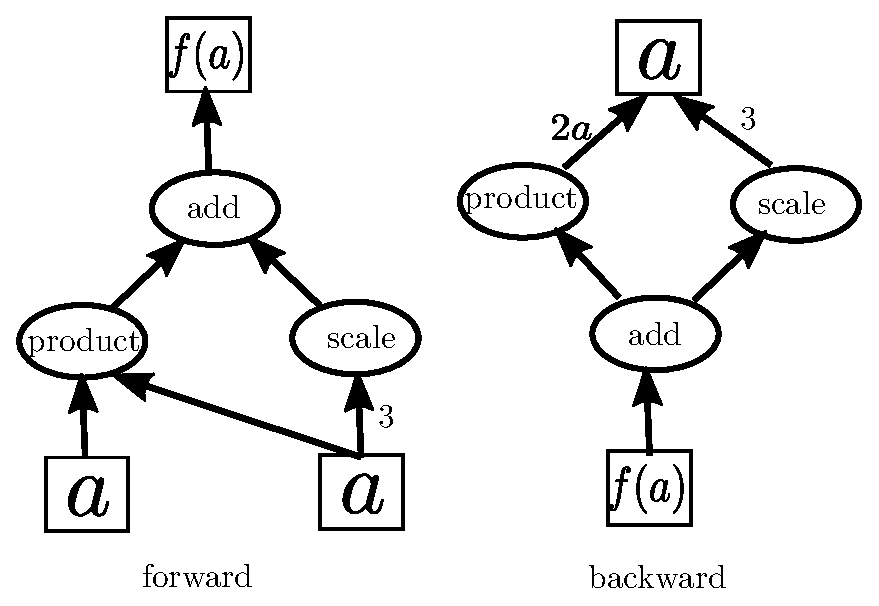
\includegraphics[width=6cm]{auto.eps}
		\end{figure}
		To implement this forward pass, we only need to implement \texttt{add}, \texttt{product}, \texttt{scale} operators and use the following pseudo Python code
		to evaluate $f(a)$ at $a=1.2$:
		\begin{lstlisting}[language=Python]
fa.eval(1.2) = s.eval(1.2) + p.eval(1.2)
s.eval(1.2) = 3 * a.eval(1.2)
p.eval(1.2) = a.eval(1.2) * a.eval(1.2)
		\end{lstlisting}
		The backward pass of $f(a)$ computes the derivative of $f$ about $a$, also illustrated in the above computational graph.
		\begin{lstlisting}[language=Python]
a.back(fa) = p.diff(a) * p.back(fa) + s.diff(a) * s.back(fa)
p.back(fa) = fa.diff(p) * fa.back(fa)
s.back(fa) = fa.diff(s) * fa.back(fa)
		\end{lstlisting}
		where \texttt{x.back(x)} is defined as identity as a convention since there is no back operation starting from self.
		The \texttt{diff} method of each tensor object computes the derivative about the adjacent variable.
		For example, \texttt{p.diff(a) = 2 * a}, \texttt{s.diff(a) = 3} etc.
		
		For multiple variable functions, the idea is the same as above but caution is needed for dimension coherence in matrix multiplication.
		
		Please implement Automatic differentiation for rank 2 tensor (matrix) based on coding template within directory \texttt{lfdnn}. To be more specific, you need to implement
		the atomic tensor object \texttt{product}, \texttt{sigmoid} and the derived tensor object \texttt{mse}. We call a tensor object
		atomic if the method \texttt{eval} and \texttt{diff} should be implemented, while a derived tensor can be treated as composition of
		atomic tensor object. You are only allowed to modify \textbf{lfdnn/operator.py}.
		
		Hint: For rank 0 tensor (scalar) or rank 1 tensor (vector), we can treat
		them as special rank 2 tensor.
		
		\question (5 points) \emph{Multilayer perceptron} You have learned Ridge Regression and softmax regression, which can be treated
		as special kind of multilayer perceptron. There are no hidden layers in these regression models and their representational power is limited.
		To represent more complex input-output relationship, we need to introduce hidden layers. For multi-class classification problems, suppose there are $k$ hidden layers,
		then the mathematical form of multilayer perceptron is as follows:
		\begin{align*}
		h_0 &= x \\
		h_i &= \sigma(w_i h_{i-1} + b_i), i = 1, \dots, k \\
		\hat{y} &= \textrm{softmax}(w h_k + b)
		\end{align*}
		We use the averaged cross entropy to define the loss function, which can also be found in WA1.2.
		\begin{align*}
		\ell(\bTheta)
		\defeq \sum_{i=1}^{m} \log p(y^{(i)}|\bm{x}^{(i)};\bTheta) = \sum_{i=1}^{m}\sum_{l=1}^{k} \bm{1}\left\{ y^{(i)} = l\right\} \log \frac{e^{\bm{\theta}_l^{\mathrm{T}}\bm{x}^{(i)}}}{\sum_{j=1}^k e^{\bm{\theta}_j^{\mathrm{T}}\bm{x}^{(i)}}}.
		\end{align*}
		
		where $\sigma$ is the activation function and $\hat{y}$ is the probability vector for each class
		We can use stochastic gradient descent to minimize $\ell(\bTheta)$, which has the following update scheme for $\ell(\bTheta)$:
		\begin{equation*}
		\ell(\bTheta)_{t+1} \leftarrow \ell(\bTheta)_t - \alpha \nabla_{\bm{\Theta}} \ell(\bTheta)_{\bm{\theta}_t}
		\end{equation*}
		where $\alpha$ is called the learning rate.
		
		To compute the gradient of the loss function, we can use the autodiff library of the first question and all forward and backward propagation details
		are hidden in the autodiff library.

		Please implement multilayer perceptron classifier by completing the code in \textbf{model.py}.
		Besides, use your MLP model to re-implement \texttt{logistic regression} in \linebreak[4] \textbf{logistic\_regression.py}, which you have already done with IRLS in PA1.
		
		\question (bonus 2.5 points) \emph{Ridge Regression with autodiff}
		Please re-implement ridge regression by completing the code in \textbf{ridge\_regression.py}, which you have already implemented with direct solution in PA1.
		You are required to use SGD with the autodiff library of question 1.

		\question (extra) \emph{Soft Margin SVM}
		Recall that soft margin SVM is solving
		the following optimization problem:
		\begin{align*}
		    \min_{w,b,\xi}& \frac{1}{2}||w||^2 + C \sum_{i=1}^m \xi_i \\
		    s.t.\, &y^{(i)} (w^T x^{(i)} + b) \geq 1 -\xi_i \\
		    &\xi_i \geq 0, i=1,\dots, m
		\end{align*}
		which can be transformed to an unconstrained
		optimization.
		\begin{equation*}
		    \min_{w, b} \frac{1}{2}||w||^2  + C\sum_{i=1}^m \max\{0, 1 - y^{(i)} (w^T x^{(i)} + b) \}
		\end{equation*}
		We can use SGD to get an approximate minimizer for the above problem.
		Please use \texttt{lfdnn} to implement soft margin SVM by completing the code in \textbf{svm.py}.		
	\end{questions}
	
	
	\nocite{*}
	\begin{flushleft}
		\textbf{Notice}: \\
		\begin{enumerate}
			\item Use matrix operations other than loops for efficiency. If the running time of Auto-Grading steps exceeds 5 minutes, you will get point deductions.
			\item You are expected to only use \texttt{numpy} packages to implement the algorithms.
			\item All questions assume that the data are not centered around zero. Therefore, you need to train the extra bias parameter in your code.
		\end{enumerate}
	\end{flushleft}
	
	%\bibliographystyle{plain}
	%\bibliography{ref}
	%\begin{thebibliography}{9}
	%	\bibitem{ridge} \href{https://ncss-wpengine.netdna-ssl.com/wp-content/themes/ncss/pdf/Procedures/NCSS/Ridge_Regression.pdf}{Ridge Regression}
	%	\bibitem{tutorial} \href{https://www.datacamp.com/community/tutorials/tutorial-ridge-lasso-elastic-net}{Regularization: Ridge, Lasso and Elastic Net}
	%\end{thebibliography}
\end{document}